\documentclass{article}
%useful packages
\usepackage[margin=1in]{geometry}
\usepackage{xeCJK}
\usepackage{helvet}
\usepackage[ruled,vlined]{algorithm2e} %for typesetting algorithms
\usepackage{graphicx}
\setCJKmainfont{Noto Sans CJK TC}
\author{Andres Ponce(0616110) \\
\and
彭思安}
\title{Introduction to Artificial Intelligence Homework 2 report}
\begin{document}

\maketitle
\section{Background}
Playing games has been an interesting research area in Artificial Intelligence
for several decades, and has led to some of the greatest accomplishments in Artificial
Intelligence, for example with Deep Blue. Several algorithms can be used to model certain types of games 
by modifying a search algorithm. One such an example is the game of Minesweeper. This game can 
be modeled by certain definite rules and thus lends itself very well to being playable by an algorithm.

In this assignment, there was a 6x6 board that consisted of three types of cells: hints, variables, and mines.
Hint nodes contain a numeric value that describes how many bombs there are in its 8 possible surrounding cells.
Given a limited number of bombs, the objective was to find a configuration of the board in which all bombs are used
and every hint node has the amount of adjacent mines described in its value. The objective was to employ
a backtracking search to carry out this search for a valid configuration. 

\section{Solution Description}
The backtracking approach used in this assignment involved a simple main algorithm:

\begin{algorithm}[H]
		\KwResult{valid board configuration}
		\caption{solve\_main(root)}
		\If{
			reject(node)
		}
		{
			return false;
		}
		\If{
			accept(node)
		}{
			return true;
		}
		make current cell mine;\\
		\For{children in node}
		{
			found = solve\_main(child);\\
			child = get\_closest\_cell(node);\\
			\If{found = true}{
					return true;\\
			}
		}
		restore cell to regular variable;\\
		return false;\\
\end{algorithm}
Following is a description of those methods.
\subsection{Rejection}
The \texttt{reject} method returns true if the valid board configuration is invalid and should be rejected, and
returns false otherwise. This method takes in a node from the board (i.e. a cell in the board with some 
additional info) and performs a simple check on adjacenthint nodes, to see if there are more mine nodes than 
the hint's value allows for. After that, we move on to the accept method.
\subsection{Accepting}
The \texttt{accept} method will check whether the current board configuration is a valid one according to the 
constraints given. For a configuration to be valid, we need both all the mines to be used up, and the hint nodes
should all have the exact amount of adjacent nodes described in their values. When this happens, then we know 
we have achieved a valid configuration. Otherwise, this method will return false.

\subsection{Recursive Step}
When the \texttt{reject} method returns, we know that placing a mine in the current cell is a valid move. So, we do that.
We change the current cell's value to that of a Mine and adjust the adjacent hint values accordingly, subtracting 1 from the 
amount of mines they can have besides them. Then, we get the $n$ closest nodes (where n is changeable) and recurse on them.
That is, we check all the configurations of the board where the current node is a mine. If it is not possible for a node to be 
a mine and arrive at a valid end configuration, then we set the current cell to a regular VAR value and return false, meaning the 
solution is not this way. 

The downside to this straightforward recursive approach is its time-complexity, which would be exponential
on the number of children $n$ each cell is allowed to check. One quick way to improve this algorithm would be to take a dynamic-
programming approach and use an array to keep track of which node configurations work. Then once we hit a node which we have previously
tested, we can know beforehand whether it leads to a possible solution or not.

\section{Testing on programs}
In this assignment, a straightforward Manhattan Distance formula is used to calculate the next node in the sequence.
The main source of additional time-complexity comes from changing the amount of chidren that a particular cell may 
have, i.e. checking the $n$ closest variable nodes which are not yet mines. Another way to calculate the next node to iterate on
would involve using other heuristics, for example MRV(by using variable nodes whose domains are now restricted),
Degree Heuristic(by measuring the amount of degrees constraining a variable), and 

For the attempt with no heuristic in place, the result was always a large amount of nodes that needed to be expanded, since any node 
could be expanded since it is only based on physical proximity to the current node. And since if the node. In some cases, this would
result in a noticeable time required for the algorithm to find a valid configuration of the board.

When attempting to modify the code to use other heuristics, there were some problems. The code was structured in such a way that 
the \texttt{get\_closest\_node()} function will simply return the next node to be expanded and remove that node from the unassigned 
queue for the time being, and if it does not lead to a valid configuration it is placed again on the unassigned queue. 
So the different heuristics were tried to be implemented as a function that retrieves a node by simply using another 
criterion for ``best", other than a simple Manhattan Distance. 

My main algorithm will pop off the node 
from the stack that is currently  being examined, and will try to assign it as a mine. Thus, at any given time in the stack there 
will be only nodes that could either be mines or variables, and thus all elements in the unassigned data structure will have a 
domain of $\{0,1\}$. 

For the degree heuristic, since we should choose the node with the less amount of constraints, then we should choose the variable 
nodes with the least amount of unassigned nodes, since these have less constraints placed on them. However, given the code structure 
already in place, and the expected revisiting of nodes given different conditions on the board made implementing a dynammic programming
solution impractical as well, since a node might not be useful given one state of the board but might be the best choice in a later one. 

For Comparison, below are the results for the sample problems given no heuristic:

\begin{center}
		\begin{tabular}{| c | c | }
				\hline
				Problem & number of expanded nodes \\ \hline
				P1 & 5374 \\ \hline
				P2 & 1892 \\ \hline
				P3 & >30,000\\ \hline
				P4  &  1843 \\
				\hline
		\end{tabular}
\end{center}

\section{Conclusion}
From the above results, it appears that the problem of quickly and efficiently using a heuristic-driven approach to Minesweeper can bring
great benefits to performance. A flexible code structure would reduce the complexity when using multiple heuristics, especially ones that
depend on different aspects of the game state, such as domains or constraints. For this specific problem, a remaining question would involve
other possible heuristics that could be used for selecting next nodes in our tree and to avoid repeated expansions of same nodes. 

This assignment has taught me about the great usefulness that heuristics bring to a more brute-force method. For some of the sample 
problems, there was a rather long wait, especially with debug messages. The sheer amount of nodes was still able to be searched rather
quickly in C++, however, for an $n x n$ board with different constraints there might be an exponentially larger delay.

With respect to other games, an area that personally appears interesting might be simulating other simple games like Minesweeper using some
heuristic-driven approach. What other games could be modeled in a similar manner? Deep Blue required special circuitry to calculate many more
possible moves in a certain amount of time. While this in impractical for most, the field of AI has come a long way, and these days there
are newer approaches to solving these problems, such as Deep Learning. It seems like a good excercise for a student to develop great 
problem-solving skills.

\section{Notes on the code base}
My program was split across several files: \texttt{main.cpp}, where the board is only input and passed on to a Board class; \texttt{Board.cpp}, 
where the files related to searching and the main algorithms are stored; and \texttt{Board.h}, where they are defined. \texttt{Util.cpp} defines 
some basic utility functions like the Manhattan Distance heuristic and check for validity of two integer coordinates $x,y$.

Since the \texttt{Board.cpp} file is quite long, I decided to include the screenshots of the main parts of the code, namely the methods described
in a prevoius section, along with \texttt{Board.h}. Sorry for the inconvenience!
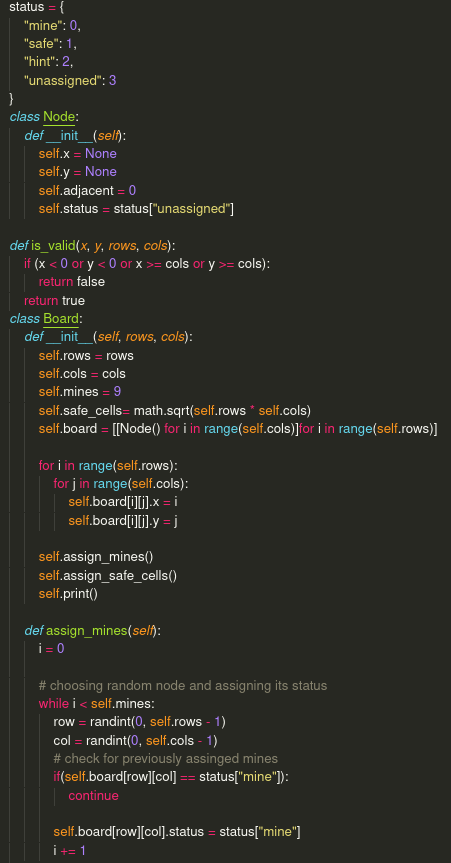
\includegraphics[scale=0.5]{../s1.png}

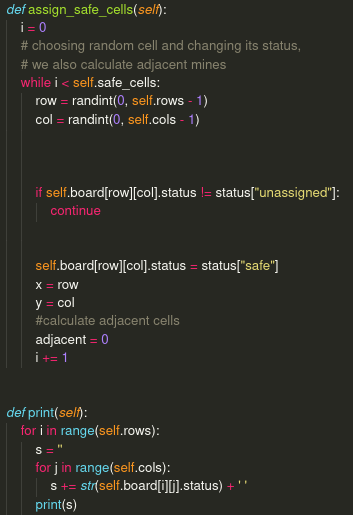
\includegraphics[scale=0.5]{../s2.png}

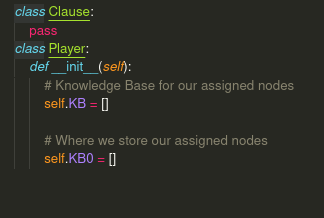
\includegraphics[scale=0.5]{../s3.png}

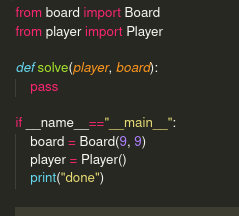
\includegraphics[scale=0.5]{../s4.png}

\includegraphics[scale=0.5]{../s5.png}
\end{document}
